%18 de marzo
\subsection{Discrete Picard's Condition}
We have already noted that $\frac{u_i^T b}{\sigma_i} \to 0$ then both $u_i^T\to 0$ and $\sigma_i\to 0$ when $i\to \infty$. \\
When we take into account the noise that goes into the exact part $b^{ex}$ that we call $\eta$. A problem arises when $\sigma_i$ keeps decaying but the numerator doesn't because it has the noise $u_i^T(b^{ex} + \eta)$ does not decay equally fast.

The Tikhonov's Regularization consists of two competing quatities: $|Lx_{reg}$ and $|Ax_{reg}-b|$. Consider the original problem $Ax=b$.
$$x_{reg}^{(l)} = \argmin \left\{ |Ax-b|^2 + l^2|Lx|^2 \right\} $$
with $l^2>0$. in general when $l$ is small $\implies$ that $|Ax-b|$ is small and $|Lx|$ is large. On the other hand if $l$ is large we would expect the opposite to happen.
\begin{center}
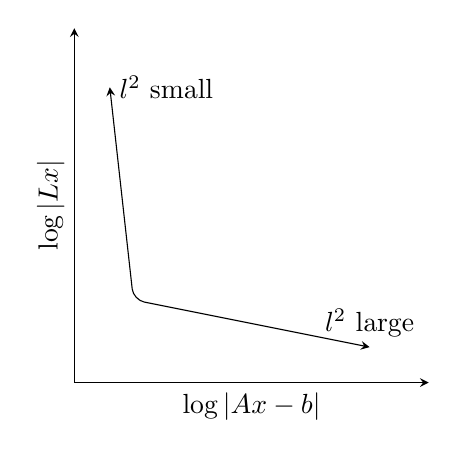
\begin{tikzpicture}[scale=1.5]
\draw [-stealth ] (0,0) -- node[below]{$\log|Ax - b|$}(3,0);
\draw [-stealth ] (0,0) -- node[sloped,above]{$\log|Lx|$}(0,3);
\draw [stealth-stealth, rounded corners ] (0.3,2.5) node[right]{$l^2$ small}-- (0.5,0.7) -- (2.5,0.3) node[above]{$l^2$ large};
\end{tikzpicture}
\end{center}

The trick is to look for the point of maximum curvature of the parametric curve $l^2$ vrs. $k=1$ and $(|Ax^{(1)} - b |, |Lx^{(1)}|)$ we will expect $|Ax-b|$ to be large.
